% Created 2022-08-14 dom 21:33
% Intended LaTeX compiler: pdflatex
\documentclass[11pt]{article}
\usepackage[utf8]{inputenc}
\usepackage[T1]{fontenc}
\usepackage{graphicx}
\usepackage{grffile}
\usepackage{longtable}
\usepackage{wrapfig}
\usepackage{rotating}
\usepackage[normalem]{ulem}
\usepackage{amsmath}
\usepackage{textcomp}
\usepackage{amssymb}
\usepackage{capt-of}
\usepackage{hyperref}
\author{Galindo}
\date{\today}
\title{}
\hypersetup{
 pdfauthor={Galindo},
 pdftitle={},
 pdfkeywords={},
 pdfsubject={},
 pdfcreator={Emacs 26.3 (Org mode 9.1.9)}, 
 pdflang={English}}
\begin{document}

\tableofcontents

\% Created 2022-08-14 dom 21:32
\% Intended \LaTeX{} compiler: pdflatex
\documentclass[12pt]{article}
\usepackage[utf8]{inputenc}
\usepackage[T1]{fontenc}
\usepackage{graphicx}
\usepackage{grffile}
\usepackage{longtable}
\usepackage{wrapfig}
\usepackage{rotating}
\usepackage[normalem]{ulem}
\usepackage{amsmath}
\usepackage{textcomp}
\usepackage{amssymb}
\usepackage{capt-of}
\usepackage{hyperref}
\newcommand{\tagline}{Práctica 1}
\newcommand{\asignatura}{Organización de Computadoras (331)}
\newcommand{\docente}{Arturo Arreola Alvarez}
\usepackage{fancyvrb}
\usepackage[spanish]{babel}
\usepackage{geometry}
\geometry{ a4paper, left=.75in, right=.75in, top=1in, bottom=1in }
\makeatletter
\renewcommand\familydefault{\sfdefault}
\usepackage{sectsty}
\sectionfont{\normalfont\huge}
\subsectionfont{\normalfont\huge}
\author\{Luis Eduardo Galindo Amaya \\
1274895\}
\date{2022-08-14}
\title\{Elementos En La Organización De Una \\
Computadora De Propósito General\}
\hypersetup\{
 pdfauthor=\{Luis Eduardo Galindo Amaya \\
1274895\},
 pdftitle=\{Elementos En La Organización De Una \\
Computadora De Propósito General\},
 pdfkeywords=\{\},
 pdfsubject=\{\},
 pdfcreator=\{Emacs 26.3 (Org mode 9.1.9)\}, 
 pdflang=\{Spanish\}\}
\begin{document}

\begin{titlepage}
  \vspace*{0.75in}
  \begin{flushleft} 
	\sffamily      
    
	\large
    \tagline \\

	\Huge
    \@title \\
    \vspace{0.25in}
    \hline
    \vspace{0.25in}
	% \vspace{0.50in}

    \Large
    \@author
    
    
    \vspace*{\fill}
	
    \large
    \begin{tabular}{ |l|l| }
      \hline
      Asignatura & \asignatura \rule{0pt}{15pt}\\
      Docente & \docente \rule{0pt}{15pt}\\
      Fecha & \@date \rule{0pt}{15pt}\\
      \hline
    \end{tabular} \\
\end{titlepage}

\setlength\parindent{0pt}   % eliminar el intentado
\setlength{\parskip}{0.75em}   % expandir el espacio entre párrafos
\vspace*{0.75in}

\section{Intrucciones}
\label{sec:org512b1be}
El alumno se familiarizará con la herramienta Marie.js para la ejecución de código en lenguaje ensamblador.

\begin{enumerate}
\item Identificar las caracteristicas de la herramienta marie.js
\begin{itemize}
\item Ingrese a la página donde se encuentra la herramienta.
\item Consulte la documentación y tutoriales de Marie, en especial las secciones Introduction to Marie y Marie Codes.
\end{itemize}

\item Realizar los programas
\begin{itemize}
\item solicite al usuario 2 números y despliegue el resultado de la ecuación \(2x+3y-5\).
\item solicite 2 números y los reste. Desplegar un 1 si el resultado fue negativo o un 0 en caso contrario.
\end{itemize}

\item Realizar un reporte que incluya: 
\begin{itemize}
\item Diagrama de bloques de una máquina de von Neumann y una breve descripción de cada componente.
\item Lista de las instrucciones de Marie y su y su función.
\item Describir el funcionamiento de los registros del Acumulador, Registro de instrucción, Contador del Programa, Registro de Acceso a Memoria (MAR), y Registro de Buffer de Memoria (MBR).
\end{itemize}
\end{enumerate}

\section{Máquina De Von Neumann}
\label{sec:org3371939}
\begin{description}
\item[{Memoria}] Son un conjunto de celdas usadas para cualquier proceso, se utiliza para almacenar los programas que va a ejecutar el procesador e información que el programa necesite almacenar.

\item[{Unidad Aritmético Lógica}] es un circuito digital electrónico que realiza las operaciones aritméticas y lógicas bit a bit en números binarios enteros.

\item[{Unidad de Control}] es un componente que dirige las operaciones del procesador. Le dice a la memoria, ALU y los dispositivos de entrada y salida cómo responder a las instrucciones de un programa.

\item[{Entrada/Salida}] Es la comunicación entre la computadora y un humano u otro sistema de procesamiento de información. Inputs son las señales o datos recibidos por el sistema y outputs son las señales o datos enviados por éste.

\item[{Registros}] son unidades de almacenamiento pequeñas que son típicamente dirigidas por mecanismos distintos de la memoria principal y a los que se puede acceder más rápido.
\end{description}

\begin{center}
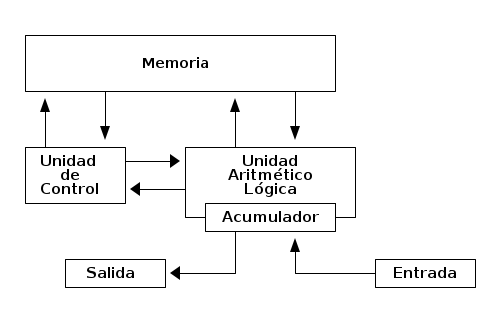
\includegraphics[width=10cm]{./img/maquina-von-neumann2.png}
\end{center}

\section{Registros}
\label{sec:orgebf4fb2}
\begin{description}
\item[{Program counter (PC)}] Registro contador del programa, contiene la dirección de la instrucción siguiente que hay que leer de la memoria.

\item[{Instruction register (IR)}] El registro de instrucción, contiene la instrucción que hay que ejecutar.

\item[{Memory address register (MAR)}] Registro de direcciones de memoria, donde ponemos la dirección de memoria a la que queremos acceder.

\item[{Memory buffer register (MBR)}] Registro de datos de memoria; registro donde la memoria deposita el dato leído o el dato que queremos escribir.

\item[{Acumulador (AC)}] el acumulador es un registro en el que son almacenados temporalmente los resultados aritméticos y lógicos intermedios que serán tratados por el circuito operacional de la unidad aritmético-lógica.
\end{description}

\section{Programa 1}
\label{sec:org915b96b}
\begin{Verbatim}[numbers=left]
INPUT                            / Captura el valor de X
Store X                          
INPUT                            / Captura un valor de Y
Store Y                          

Clear                            / limpiar Acumulador, hacer AC ← 0

Add X                            / 2x
Add X 
Add Y                            / 3y
Add Y
Add Y
Subt R                           / -5

Output
Halt

X, DEC 0
Y, DEC 0
R, DEC 5
\end{verbatim}
\end{document}
\end{document}
